La structure des différents dossiers faisant partie du projet est la suivante (affichage via la commande tree -d dans le terminal) :

\begin{figure}[H]
\centering
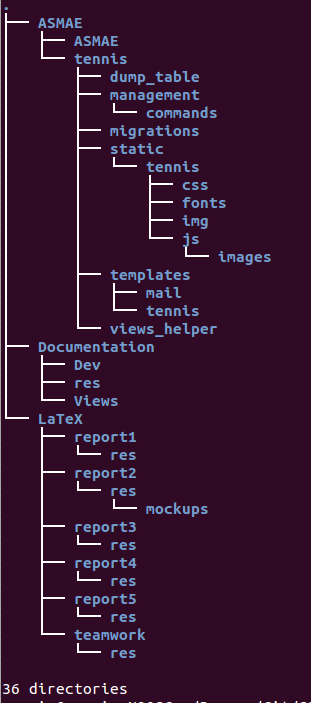
\includegraphics[scale=0.45]{Tree.png}
\caption{Arbre décrivant l'architecture du répertoire}
\end{figure}

Le répertoire du projet se sépare en 3 sous-dossiers :

\begin{itemize}
\item un dossier "ASMAE" contenant les fichiers propres à la création du site web,
\item un dossier "Latex" contenant les différents rapports intermédiaires remis lors de la période de développement,
\item et un dossier "Documentation" contenant les textes et images faisant parties de l'aide à l'utilisation du site.
\end{itemize}

\begin{figure}[H]
\centering
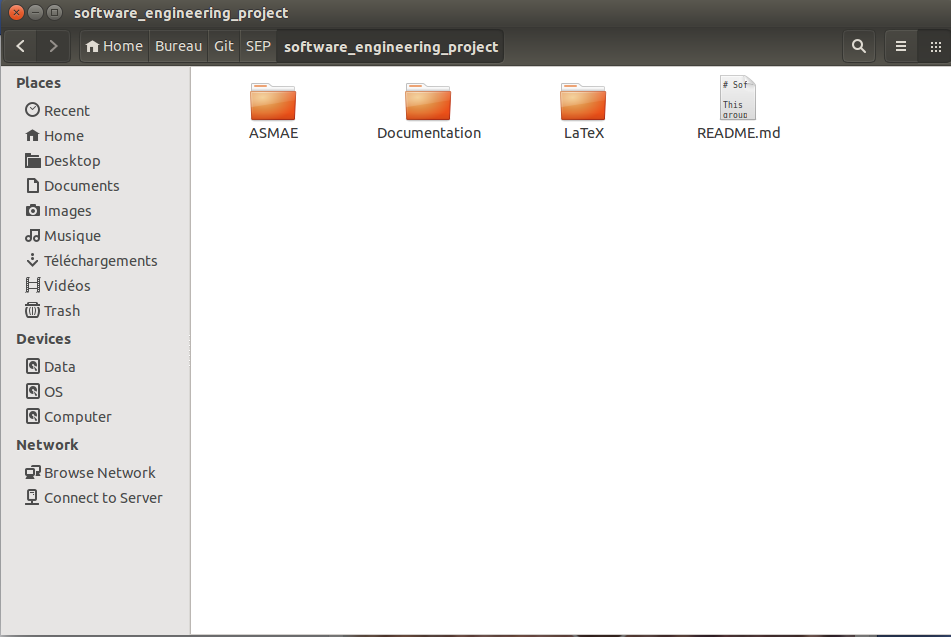
\includegraphics[scale=0.35]{Repository.png}
\caption{Architecture du répertoire}
\end{figure}

\begin{figure}[H]
\centering
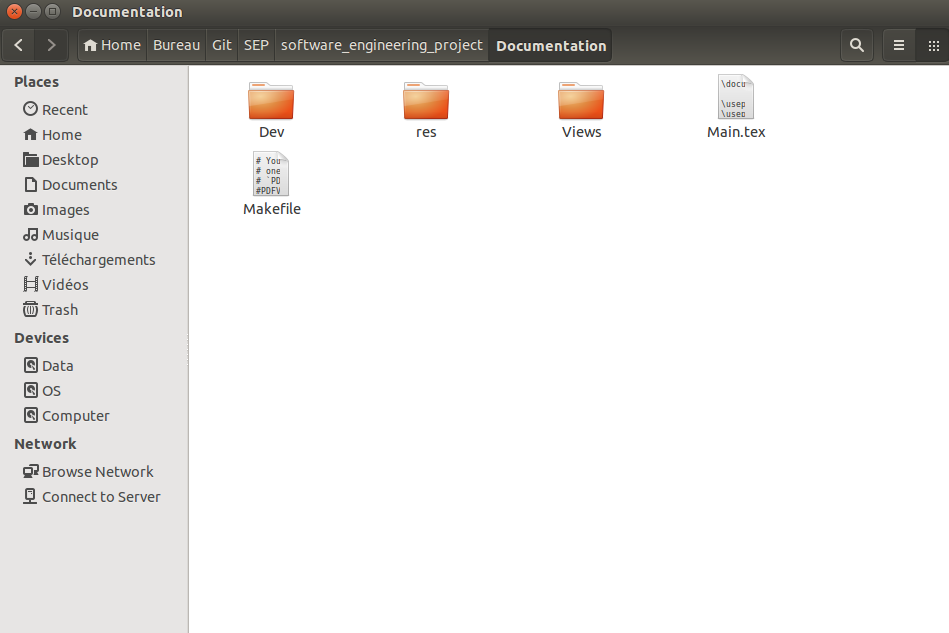
\includegraphics[scale=0.35]{Documentation.png}
\caption{Documentation}
\end{figure}

\begin{figure}[H]
\centering
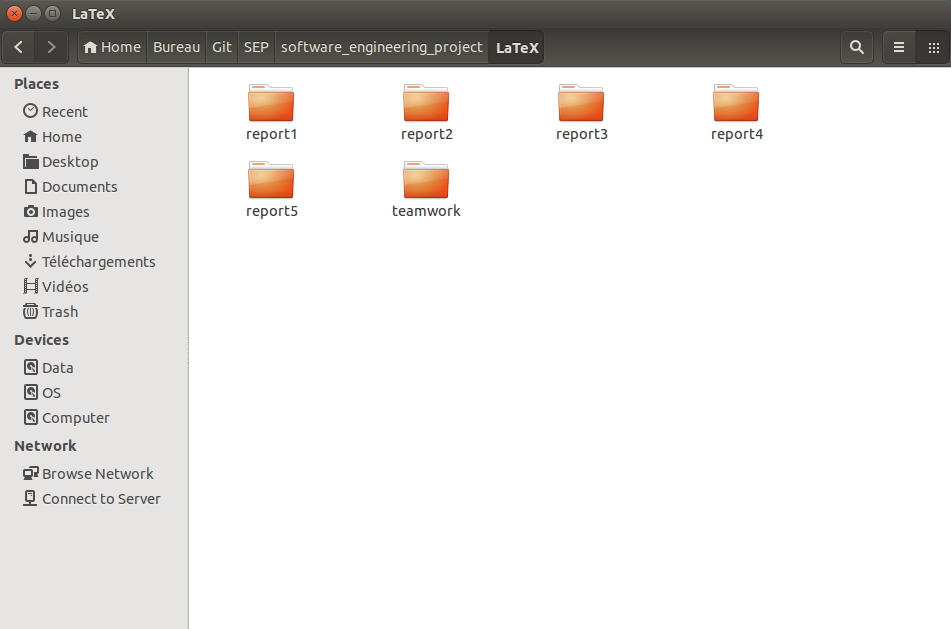
\includegraphics[scale=0.35]{Latex.png}
\caption{Dossier Latex}
\end{figure}

Dossier ASMAE:\\

A l'ouverture de ce dossier, on retrouve à nouveaux deux sous-dossiers :\\

\begin{itemize}
	\item le dossier "ASMAE" contient  la base de données ainsi que trois fichiers se rapportant à la configuration de Django (settings.py pour les options de Django, urls.py pour lier les views aux templates et wsgi.py pour définir l'application web), 
	\item le dossier "tennis" contenant l'ensemble des ressources du site internet. On y retrouve également plusieurs fichiers :
	\begin{itemize}
		\item un fichier manage.py permettant d'interragir directement avec l'application (lancer le site web, créer un superuser, effectuer les migrations de la base de données, …), 
		\item deux fichiers textes (res\_femmes.csv et res\_hommes.csv) reprenant les informations des utilsateurs hommes et femmes utilisés pour populer la base de données, 
		\item et un fichier exécutable phantom.js utilisé quant à lui pour la gestion des envois d'email du site web.
	\end{itemize}
\end{itemize}

\begin{figure}[H]
\centering
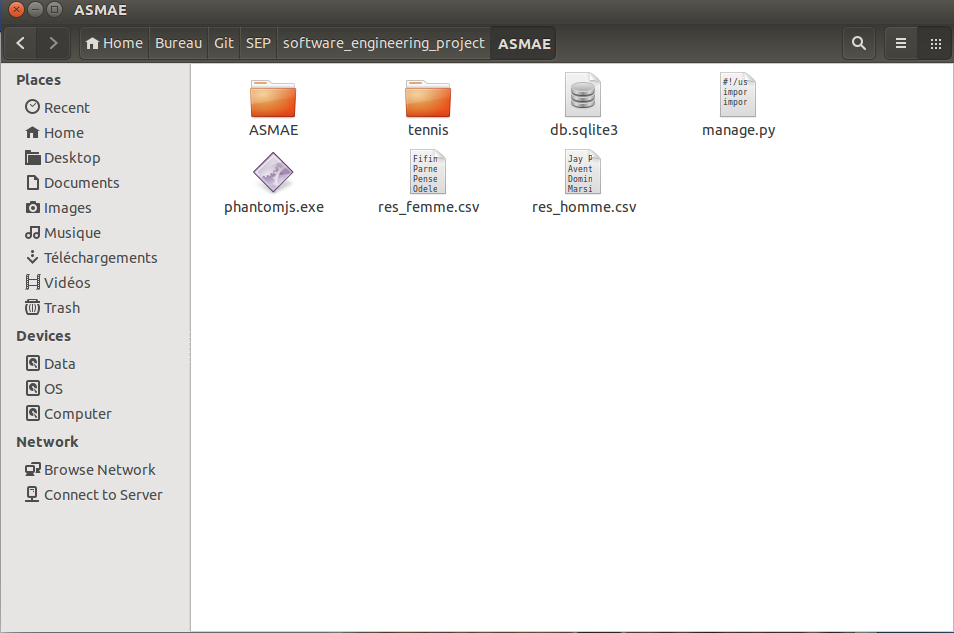
\includegraphics[scale=0.35]{Asmae1.png}
\caption{Dossier Asmae 1}
\end{figure}
\vspace{-5cm}
\begin{figure}[H]
\centering
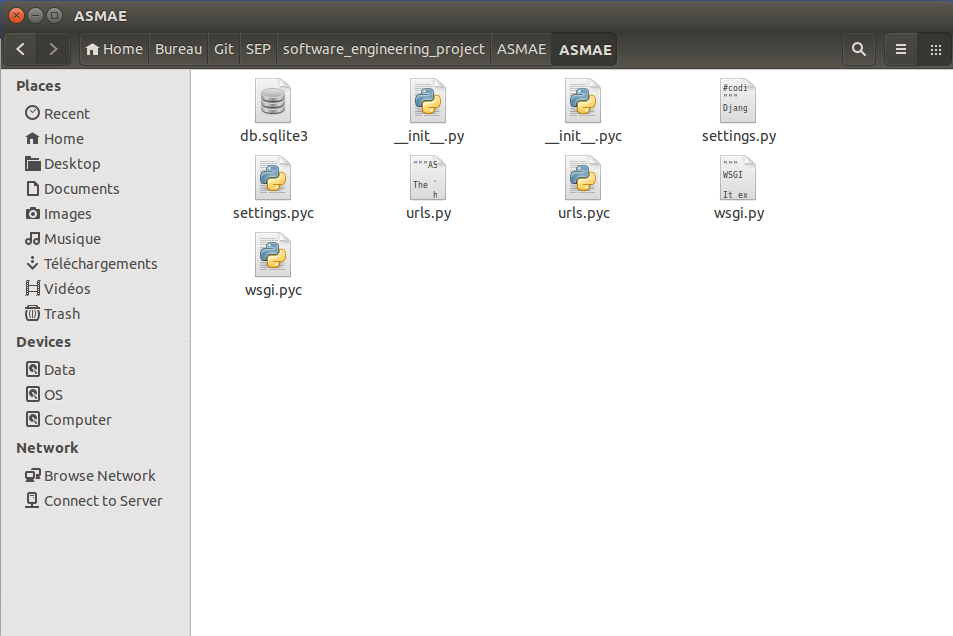
\includegraphics[scale=0.35]{Asmae2.png}
\caption{Dossier Asmae 2}
\end{figure}

Dossier tennis :\\

C'est dans ce dossier que se trouvent toutes les ressources principales du projet. On y retrouve les dossiers suivants :
\begin{itemize}
	\item le dossier "dump\_table" qui reprend le code permettant de transférer les différents terrains (courts.py) et joueurs (participant.py) de la base de données vers des fichiers texte (.csv),
	\item le dossier "management" qui reprend le code de tous les formulaires utilisés sur le site (dans le sous-dossier "commands") ainsi que deux fichiers texte (.csv) contenant les utilisateurs hommes et femmes utilisés pour populer la base de données et un fichier contenant le code permettant de créer un utilisateur aléatoire (random\_people.py),
	\item le dossier "migrations", contenant toutes les migrations effectuées de la base de données,
	\item le dossier "static" contenant toutes les ressources statiques utilisées par le site web (les fichiers css, les polices, les images et le code javascript),
	\item le dossier "templates" contenant toutes les pages HTML du site ainsi que les templates utilisés pour les mails des membres du staff (dans le sous-dossier "mails"),
	\item et le dossier "views\_helper" qui reprend l'implémentation de certaines views particulières (comme l'encodage par un utilisateur de ses points dans la poule, ou encore d'accepter ou de refuser une demande d'un autre utilisateur pour former une paire).\\
\end{itemize}

On retrouve également les fichiers suivants :\\

\begin{itemize}
	\item le fichier admin.py qui contient le code définissant les différentes classes des administrateurs (administrateur s'occupant des tournois, des terrains, ...) ainsi que leurs attributs, utilisés pour créer les tables dans la base de données,
	\item le fichier classement.py qui contient le code permettant de faire le classement des différents participants dans les poules,
	\item le fichier forms.py qui contient le formulaire de connexion au site,
	\item le fichier mail.py qui contient le code nécessaire à l'envoi des différents types de mails (confirmation d'enregistrement, paiement, ...) du site,
	\item le fichier models.py qui contient le code définissant les différentes classes (participant, terrain, ...) ainsi que leurs attributs, utilisés pour créer les tables dans la base de données,
	\item le fichier pdfdocument.py qui contient le code utilisé pour la transformation des pages du site en fichier pdf imprimable, 
	\item le fichier tests.py qui contient les différents tests des fonctionnalités du site que nous avons implémentés,
	\item le fichier urls.py qui contient toutes les URL disponibles sur le site, et leurs liens vers les views contenues dans le fichier views.py
	\item et le fichier views.py qui contient l'ensemble des views présentes sur le site.
\end{itemize}

\begin{figure}[H]
\centering
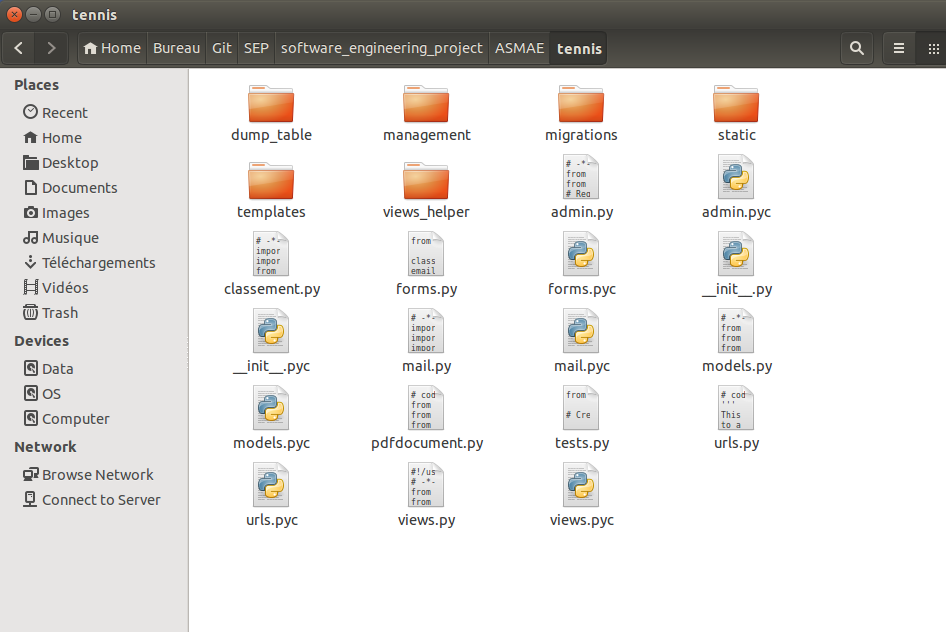
\includegraphics[scale=0.35]{tennis.png}
\caption{Dossier tennis}
\end{figure}
